\section{Vecinos más cercanos}

% \todo[inline]{Como esta representada nuestra informacion}
% Todas las imágenes de nuestro set de datos tiene una dimensión de 28x28 píxeles (En total 784 píxeles). Al cargar una imagen, la guardaremos como un vector de 784 coordenadas. Y BLAH

Nuestro problema consiste en tomar una imagen de un dígito manuscrito, y decidir cuál es el dígito que representa. Escrituras de un mismo dígito para distintas personas pueden ser muy diferentes entre sí, e incluso en ocasiones puede ser complicado para un ser humano distinguirlos. \\

{\centering
    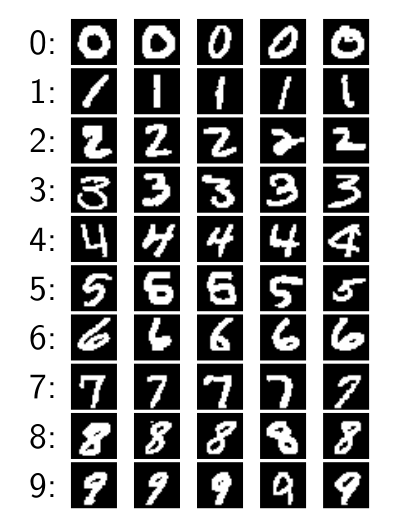
\includegraphics[scale=0.40]{informe/imagenes/knn/muestraVariaciones.png} \\
    \captionof{figure}{Algunas muestras diferentes para los mismos dígitos. \\
    (Fuente de imagen: Clase de laboratorio) \\ }
}
$ $\newline

El primer método que presentaremos para resolver este problema, es el método de \textit{k-Vecinos más cercanos}, o en inglés \textit{k-Nearest Neighbors}. De ahora en más utilizaremos indistintamente el nombre \textbf{kNN} por sus siglas en inglés. \\

Tenemos diez categorias posibles (los dígitos 0-9) y un conjunto de imágenes para las cuáles conocemos el dígito que representan. Llamaremos a este conjunto de imágenes el \textit{conjunto de datos etiquetados}. Dado un nuevo dato \textbf{sin etiquetar}, queremos decidir a qué categoría pertenece. La forma más natural para clasificarlo, es compararlo con nuestros datos conocidos y elegir la categoría a la cuál más se \textit{parezca}. \textit{kNN} es una implementación y una generalización de esta idea. \\

Dado que nuestras imágenes son en realidad vectores en $\mathbb{R}^{784}$ (pues sus dimensiones son 28x28 píxels), utilizaremos la diferencia en norma entre dos vectores para cuantificar qué tan \textit{parecidas} son dos imágenes. Dicho de otro modo, consideramos que dos imágenes son parecidas cuando los vectores que las representan son cercanos en norma. \\

La idea fundamental es que grupos de imágenes similares estarán cercanas entre sí, por lo que al querer identificar una imagen desconocida, nos basta con ver cuál es la categoría de las imagenes cercanas. Dado que existe la posibilidad de \textit{outliers}, o que la imagen caiga cerca del límite entre dos grupos, no tomaremos la única imagen mas cercana sino que consideraremos el conjunto de las \textit{k} más cercanas. \\

\todo[inline]{Usar alguna imagen ilustrativa}


$ $\newline

Como detalles de implementación, intentamos siempre minimizar la cantidad de operaciones y evitar el pasaje de variabels por copias. Además, para tomar los $k$ de menor distancia utilizamos un \textit{min-heap} que tiene una complejidad menor que las alternativas. Esto es interesante considerar pues la cantidad de iteraciones depende fuertemente del tamaño de $n$, mientras que $k$ en general es pequeño.\\

Aquí algunas de las alternativas consideradas para la elección de los $k$ menores, con $n$: cantidad de imágenes.

\begin{enumerate}
\item $O$($n * k$) : Realizar $k$ pasadas tomando el mínimo en cada una.
\item $O$($n * log(n)$) : Ordenar todos y tomar los primeros $k$.
\item $O$($n * log(k)$) : Tomar los $k$ menores con un min-heap.
\end{enumerate}

Si fijamos por ejemplo $k = 25$ y $n = 42000$ (n maximo), podemos realizar el siguiente cuadro:

\begin{center}
    \begin{tabular}{| c | c |}
    \hline
    Complejidad   &  Cantidad de comparaciones estimada \\ \hline

    $O$($n * k$)            & 1050000  \\ \hline
    $O$($n * log(n)$)       & 644700  \\ \hline
    $O$($n * log(k)$)       & 194880   \\ \hline
    \end{tabular}
\end{center}

Aunque quizá un millón de comparaciones no parece excesivo, es importante aclarar que cada comparación consiste en ver componente a componente las diferencias entre vectores, dónde cada vector tiene 728 componentes. Además, esto es para el caso de clasificar una única imagen. Si queremos clasificar muchas imágenes deberíamos repetir el procedimiento para cada una de ellas, y si consideramos que la base de Kaggle tiene más de 20000 imágenes para clasificar, optimizar el método no es algo menor. \\


\todo[inline]{TODO: Estaria bueno en la experimentacion hacer una medicion de tiempos entre posibles implementaciones de knn.}

Tendría mucho sentido explorar algún método que reduzca el costo de las comparaciones. En la siguiente sección presentaremos un método que analiza sólo las componentes principales de nuestros vectores en vez de las 728 ya mencionadas. En la sección de experimentación realizaremos comparaciones entre ambos métodos. \\


\section{PCA}

En esta sección hablaremos sobre el método de \textit{Principal Component Analysis} (en español, análisis de componentes principales). El problema que teníamos con el método anterior es la gran cantidad de dimensiones con las que teníamos que lidiar. Este método lo que intenta es reducir la dimensionalidad de un conjunto de datos, quedandose únicamente con aquellas dimensiones más significativas. Podemos considerar que las dimensiones de nuestro espacio son las componentes de la muestra, por lo tanto, estamos buscando justamente las componentes principales. \\

% Che alto copypaste de wikipedia
% Supongamos que existe una muestra con n individuos para cada uno de los cuales se han medido m variables (aleatorias) $F_{j}$. El PCA permite encontrar un número de factores subyacentes p $<$ m que explican aproximadamente el valor de las m variables para cada individuo. El hecho de que existan estos p factores subyacentes puede interpretarse como una reducción de la dimensionalidad de los datos: donde antes necesitabamos m valores para caracterizar a cada individuo ahora nos bastan p valores. Cada uno de los p encontrados se llama componente principal, de ahí el nombre del método. \\
% El PCA construye una transformación lineal que escoge un nuevo sistema de coordenadas para el conjunto original de datos en el cual la varianza de mayor tamaño del conjunto de datos es capturada en el primer eje (llamado el Primer Componente Principal), la segunda varianza más grande es el segundo eje, y así sucesivamente. Para construir esta transformación lineal debe construirse primero la matriz de covarianza . Como esta matriz es simetrica (ya que la covarianza entre A y B es igual a la covarianza entre B y A) sabemos que existe una base ortonormal de autovectores . La transformación que lleva de las antiguas coordenadas a las coordenadas de la nueva base es precisamente la transformación lineal necesaria para reducir la dimensionalidad de datos. \\

Sea $\{ x_i : i = 1 .. n\}$ nuestro conjunto de imágenes.  \\

Lo primero que haremos será normalizar nuestro conjunto de datos. Para esto definimos la media $\mu$:
$$ \mu = (x_1 + x_2 + .. + x_n) / n $$

Definimos entonces la matrix $X \in \mathbb{R}^{n x m}$ como la matriz que contiene en la fila $i$ al vector:

$$ (x_i - \mu)^{t} / \sqrt{n-1} \hspace{1cm}(1) $$

La matriz $X$ contiene todos nuestros datos normalizados. Para encontrar componentes principales debemos analizar cómo están relacionadas las diferentes componentes entre sí. Para esto consideraremos la matriz de covarianzas:

$$M_x = X^t X$$

El siguiente paso será diagonalizar $M_x$. Esto es posible ya que la matriz de covarianzas es simpetrica, por lo que sus autovectores forman una base ornotormal. Lo que logramos con esto es que la varianza de cada variable quede expresada en la diagonal, y como en la diagonal encontraremos valores positivos (pues es simétrica) ordenados de mayor a menor, sus autovectores asociados representarán las componentes principales.

$$ M_x = V^t D V$$

Debido a que nos interesan únicamente las componentes principales, podemos tomar de $V^t$ las primeras $alpha$ componentes y utilizarlas como una matriz de cambio de base. \\

Para finalizar, a cada una de nuestras muestras les aplicamos el proceso de normalización expuesto en (1), y luego le aplicamos el cambio de base que acabamos de conseguir. Cuándo querramos clasificar una nueva imagen, también debemos normalizarla y aplicarle la transformación. \\

Este método logra reducir la dimensión de nuestros datos, por lo que cuando elijamos los k vecinos más cercanos en este nuevo espacio, estaremos haciendo comparaciones únicamente con las componentes principales, por lo que estaríamos reduciendo el tiempo de cómputo considerablemente. Veremos más adelante si esta disminución de dimensión empeora los resultados obtenidos. \\

Para poder hacer uso de este método tendremos que hacer un cálculo de autovectores, para esto utilizaremos el método de la potencia y el método de deflación, ambos explicados en la siguiente sección. \\

Un problema que surgió con la implementación es que el cálculo de la matriz de covarianzas y su diagonalización resulta costoso. Si queremos experimentar para diferentes $k$ esto resulta problemático. Por este motivo, en nuestros experimentos, aprovechamos que si sólo variamos el $k$ la matriz de cambio de base se mantiene igual guardando nuestras matrices de cambio de base en como csv para simplemente cargarla si ya fué calculada. \\

\section{Método de la potencia y Deflación}

Cómo habíamos mencionado, para poder diagonalizar la matriz de covarianza necesitamos conseguir los autovalores y autovectores. Conseguir los autovalores de la manera tradicional implica encontrar las raíces de un polinomio de grado 784, y no es algo que estemos dispuestos a intentar. Utilizaremos entonces el método iterativo conocido como \textit{Método de la potencia}.
\begin{algorithm}
    \caption{Método de la potencia (Matriz $B$, Vector $x_0$, Int $iters$)}
    \begin{algorithmic}[h]
        \State{$v \gets x_0$}
        \For{$i \gets 1$ to $iters$}
            \State{$v \gets \frac{Bv}{\norm{Bv}}$} \\
        \EndFor
        \State  $\lambda \gets \frac{v^tBv}{v^tv}$
        \State return $(\lambda, v)$

    \end{algorithmic}
\end{algorithm}

Podemos estar seguros de que los autovalores son números reales positivos, pues la matriz de covarianza es una matriz simétrica. Además, también por ser simétrica sabemos que vamos a poder conseguir una base de autovectores ortonormales, que es exactamente lo que necesitamos. \\

Con el método de la potencia conseguimos únicamente el autovalor dominante (y un autovector correspondiente). Como queremos conseguir una base, extendemos el método de la potencia utilizando el método de deflación. Esto funciona por la siguiente observación:

$$ B - \lambda v_1 {v_1}^{t} \text{\hspace{1cm}tiene los mismos autovalores que B (excepto $\lambda$).} $$

Por lo tanto, cuando apliquemos el método de la potencia en la matriz resultante, el autovalor que conseguiremos será distinto del $\lambda$ obtenido inicialmente. \\

Otro detalle es que el vector inicial $x_0$ es elegido aleatoriamente. Si bien es posible en teoría que con un cierto $x_0$ el método no converja, en la práctica eso no sucede. En primer lugar, hay muy pocas probabilidades de tomarlo, y en segundo lugar, los errores de precisión juegan a nuestro favor, ya que con una mínima desviación el $x_0$ deja de ser problemático. \\

El último factor a tener en cuenta es la cantidad de iteraciones para la convergencia. Para que pasen los tests de la cátedra es necesario hacer más de 1000 iteraciones. Sin embargo, como veremos en la sección de experimentación, con una cantidad muchísimo menor de iteraciones el accuaracy obtenido no se modifica, por lo que tomaremos una cantidad mucho menor de iteraciones para optimizar el tiempo de ejecución. \\

\section{K-Fold Cross Validation}

A lo largo de la experimentación, entrenaremos nuestro sistema con un cierto conjunto de datos y luego clasificaremos muestras. Como queremos saber qué tan bien o qué tan mal funciona nuestra sistema, estas muestras estarán etiquetadas para poder comparar el grupo real con el grupo predicho. \\

Dado que nuestra base de información es, si bien extensa, limitada, surge la pregunta de cómo elegir cuáles datos entrenar y cuáles clasificar. Más aún, si tomamos siempre los mismos datos, los mejores parámetros que obtengamos serán para ese set de datos en particular, y esto no es algo deseable (el problema mencionado es conocido como \textit{overfitting}). Para resolver estas problemáticas, utilizaremos la técnica de \textit{K-Fold Cross Validation}. \\

El método consiste en particionar nuestro espacio de muestras en $K$ grupos (a partir de ahora, \textit{folds}) y utilizar $K - 1$ folds como datos de entrenamiendo y el fold restante para testeo. Fijados $K$ y los demás parámetros necesarios para nuestro entrenamiento, ejecutaremos el método $K$ veces, donde en cada iteración se varía cuál es el fold que se utilizará para testear. Al finalizar cada iteración se obtendrá un valor correspondiente a cierta métrica (por ejemplo $accuaracy$) y el resultado final será el promedio de todas las iteraciones. \\

{\centering
    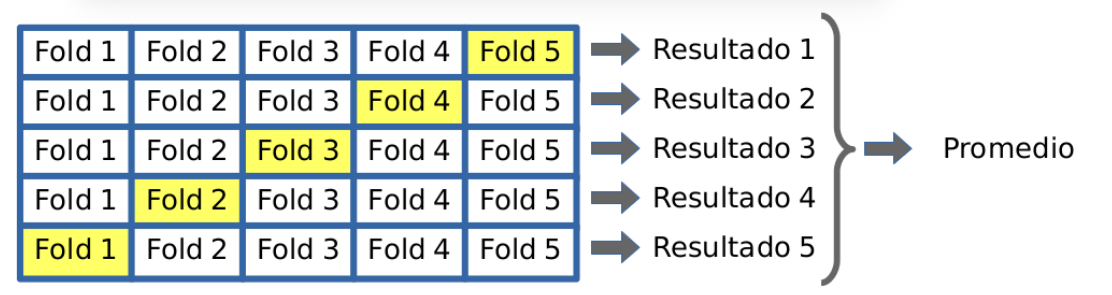
\includegraphics[scale=0.30]{informe/imagenes/kfold/kfoldEjemplo2.png} \\
    \captionof{figure}{Ejemplo de K-fold con K = 5. \\
    (Fuente de imagen: Clase de laboratorio) \\ }
}
$ $\newline
Dado que nuestra clasificación no es binaria, los datos que obtendremos serán para cada una de las 10 categorías, y la efectividad de los parámetros se analizará por separado. Es posible que nuestro clasificador sea muy bueno para ciertos dígitos pero que sea malo para otros. \\

\todo[inline]{No se si vale la pena mencionar la implementacion, pensar que mas}


